\documentclass[11pt,a4paper]{article}

\usepackage[utf8]{inputenc}
\usepackage[T1]{fontenc}
\usepackage[margin=2.2cm]{geometry}
\usepackage{amsmath,amssymb}
\usepackage{booktabs}
\usepackage{longtable}
\usepackage{tabularx}
\usepackage{array}
\usepackage{float}
\usepackage{xcolor}
\usepackage{enumitem}
\usepackage{fancyhdr}
\usepackage{caption}
\usepackage{tikz}
\usetikzlibrary{arrows.meta,positioning,shapes.geometric,calc}
\usepackage[colorlinks=true,linkcolor=navy,urlcolor=tealblue,citecolor=navy,plainpages=false,pdfpagelabels]{hyperref}
\sloppy

\definecolor{navy}{RGB}{20,56,110}
\definecolor{tealblue}{RGB}{15,108,140}
\definecolor{lightgraybg}{RGB}{246,248,251}

\pagestyle{fancy}
\fancyhf{}
\rhead{\small\color{gray} Technical documentation and presentation Q\&A}
\cfoot{\small\thepage}
\renewcommand{\headrulewidth}{0.4pt}

\newcommand{\code}[1]{\texttt{#1}}
\emergencystretch=1.5em
\newenvironment{qa}[1]{%
  \par\medskip\noindent\textbf{\color{navy}#1}\par\smallskip\noindent\ignorespaces
}{\par\medskip}

\begin{document}
\pagenumbering{roman}

% ----------------------------------------------------------------------
% TITLE PAGE
% ----------------------------------------------------------------------
\begin{titlepage}
  \thispagestyle{empty}
  \centering
  \vspace*{1.0cm}
  {\small\textsc{Alma Mater Studiorum, Universit\`a di Bologna}\par}
  {\small Dipartimento di Informatica, Scienza e Ingegneria (DISI)\par}
  \vspace{1.2cm}

  {\Huge\bfseries\color{navy} Music-synchronized AI choreography planning for the humanoid NAO robot\par}
  \vspace{0.5cm}
  {\Large\color{tealblue} Architecture, heuristic search, simulator stabilization, and oral defense guide\par}
  \vspace{1.0cm}

  {\small
  \begin{tabularx}{0.96\textwidth}{r X}
    \toprule
    \textbf{Course} & Fundamentals of Artificial Intelligence (NAO Planning Competition) \\
    \textbf{Team members} & {[Team Member 1, Email]} \\
                          & {[Team Member 2, Email]} \\
    \textbf{Repository} & \url{https://github.com/KOlCIqwq/NAO} \\
    \textbf{Audio track} & Rick Astley, \emph{Never Gonna Give You Up} (113.3\,BPM; WAV 120.0\,s, MP3 120.12\,s) \\
    \textbf{Target platform} & SoftBank Robotics NAO H25, Choregraphe Suite 2.8 (Python 2.7 / 3.x) \\
    \bottomrule
  \end{tabularx}
  }

  \vspace{1.2cm}
  \begin{abstract}
    \noindent This document explains how our NAO Planning Competition entry works and why we made each design choice. Instead of writing a fixed list of moves or scoring moves by hand, we split the project into three Python scripts. First, \code{audio\_analyzer.py} reads 16-bit PCM WAV samples to measure how loud each musical bar is, where volume dips happen, and which bars repeat as verses or choruses. Next, \code{nao\_planner.py} reads joint angles from 37 move scripts in \code{RobotPositions/} and runs forward state-space A* search to build \code{choreography\_plan.json}. Finally, \code{execute\_choreography.py} wraps NAOqi proxies at runtime so the robot stays on the beat inside Choregraphe, avoids falling during sitting and standing moves, and finishes under 120\,s. Across the 37 candidate moves, \code{ChoreographyPlanner.solve()} expands 8,937 nodes in 0.077\,s (0.71\,s total including file loading) and finds a 29-step, 111.0\,s plan at cost 181.85. A live run on Choregraphe Suite 2.8 (port 9559) finished in 115.4\,s with zero errors, ended in \code{Crouch} (\code{HeadZ = 0.354\,m}), and stopped at odometry coordinates $x = -0.004\,\text{m}$, $y = +0.009\,\text{m}$ ($\theta = -0.177\,\text{rad}$).
  \end{abstract}

  \vfill
  {\small\color{gray} Prepared for project submission and voting-day presentation.\par}
\end{titlepage}

\tableofcontents
\newpage
\pagenumbering{arabic}

% ----------------------------------------------------------------------
% SECTION 1: EXECUTIVE SUMMARY
% ----------------------------------------------------------------------
\section{Executive summary}

Our system splits audio analysis, move planning, and robot execution into three separate scripts. Each piece can be run and tested on its own.

\code{audio\_analyzer.py} reads \code{rick\_120s.wav} (56 bars at 113.3\,BPM, starting at phase 0.21\,s) and scores each bar's loudness on a 1.0 to 5.0 scale. It also flags bars with sudden beat-level volume drops and groups 4-bar phrases into sections. It needs only the Python standard library, and falls back to an MP3 parser or a generic structure curve when no WAV file is available. If \code{numpy} and \code{scipy} are installed, \code{detect\_tempo\_and\_beats()} can also estimate BPM from WAV files.

\code{nao\_planner.py} inspects 37 configured move scripts inside \code{RobotPositions/} (out of 58 Python files in that folder) to measure their duration, joint speed, motion range, pauses, and start/end poses. It then runs forward state-space A* search. The search tracks the 6 mandatory moves with a 6-bit mask rather than locking them into one order, picks at least 5 official intermediate moves from Slides 16 and 17, tracks stage movement, and chooses moves that fit the song's energy and beat.

\code{execute\_choreography.py} runs \code{choreography\_plan.json} on a virtual or physical NAO robot. It wraps \code{ALMotion}, \code{ALRobotPosture}, and \code{ALTextToSpeech} at runtime so the robot stays synced to the music even when Choregraphe lags, uses safe joint angles during \code{Sit}, \code{SitRelax}, and \code{Stand}, skips post-speech pauses without dropping real movement delays, and skips late optional motifs if wall time gets close to 120\,s.

Table~\ref{tab:verification} summarizes the headline verification metrics recorded during our live test on Choregraphe Suite 2.8.

\begin{table}[H]
  \centering
  \small
  \caption{Measured verification results on live Choregraphe Suite 2.8 (port 9559).}
  \label{tab:verification}
  \begin{tabularx}{\textwidth}{l X}
    \toprule
    \textbf{Metric} & \textbf{Observed value} \\
    \midrule
    Candidate pool size & 37 configured moves (1 initial, 1 goal, 6 mandatory, 29 intermediate) \\
    Planner runtime & 0.077\,s for \code{solve()} alone; 0.71\,s full pipeline (Python 3) \\
    A* search stats & 8,937 expanded nodes, 181.85 regret cost (identical on Python 2.7 and 3.x) \\
    Planned sequence & 29 moves, 111.0\,s nominal total, 5 official intermediate moves \\
    Live simulation run & 115.4\,s actual wall time ($< 120.0\,\text{s}$ cap), 0 runtime errors \\
    Mandatory moves executed & 6 / 6 (\code{WipeForehead}, \code{Hello}, \code{15-StandZero}, \code{16-Sit}, \code{17-SitRelax}, \code{11-Stand}) \\
    Official intermediate moves & 5 / 5 (\code{3-Double\_movement}, \code{sprinkler}, \code{4-Arms\_opening}, \code{8-Move\_backward}, \code{7-Move\_forward}) \\
    Final robot state & \code{Posture = Crouch}, \code{Family = Crouching}, \code{HeadZ = 0.354\,m} \\
    Final odometry reading & $x = -0.004\,\text{m}$, $y = +0.009\,\text{m}$, $\theta = -0.177\,\text{rad}$ \\
    \bottomrule
  \end{tabularx}
\end{table}

\clearpage

% ----------------------------------------------------------------------
% SECTION 2: COMPETITION REQUIREMENTS AND COMPLIANCE
% ----------------------------------------------------------------------
\section{Competition requirements and compliance}

We verified our system against both the hard technical rules and the qualitative evaluation criteria in \code{NAOPlanningChallenge2627.pdf}. The sections below detail our compliance checklist and alignment with the voting-day survey questions.

\subsection{Hard rules checklist (Slides 10 to 20)}

Table~\ref{tab:rules} matches each rule from \code{NAOPlanningChallenge2627.pdf} to our code and to what happened in our live Choregraphe test.

\begin{table}[H]
  \centering
  \small
  \caption{Compliance matrix against competition rules.}
  \label{tab:rules}
  \begin{tabularx}{\textwidth}{>{\raggedright\arraybackslash}p{3.4cm} >{\raggedright\arraybackslash}p{4.2cm} X}
    \toprule
    \textbf{Requirement} & \textbf{Code enforcement} & \textbf{Verified outcome} \\
    \midrule
    Initial state: \code{StandInit} (Slide 12) & \code{INITIAL\_SPEC = "14-StandInit.py"} & Step 1 wakes the robot and enters \code{StandInit}. \\
    Goal state: \code{Crouch} (Slide 12) & \code{GOAL\_SPEC = "6-Crouch.py"} & Step 29 finishes in \code{Posture = Crouch} (\code{HeadZ = 0.354\,m}). \\
    6 mandatory positions (Slide 13) & 6-bit mask \code{mand\_mask == 63} & All 6 run: \code{WipeForehead}, \code{Hello}, \code{15-StandZero}, \code{16-Sit}, \code{17-SitRelax}, \code{11-Stand}. \\
    At least 5 official intermediate moves (Slides 14 to 17) & \code{off\_cnt >= 5} in goal test; \code{official=True} flags & 5 official moves chosen: \code{3-Double\_movement}, \code{sprinkler}, \code{4-Arms\_opening}, \code{8-Move\_backward}, \code{7-Move\_forward}. \\
    Consecutive incompatibilities (Slide 14) & Posture states, floor order, static-move guard & \code{16-Sit} requires \code{Standing} at $(0,0)$; \code{11-Stand} requires \code{17-SitRelax}; sitting moves match \code{Sitting}. \\
    Time limit of 2 minutes (Slides 10, 15, 18) & \code{max\_duration = 115.0\,s}; runtime \code{MAX\_WALL\_TIME = 115.5\,s} & Planned 111.0\,s; live Choregraphe run finished in 115.4\,s. \\
    Cross-platform execution (Slide 10) & Stdlib planner; multi-OS audio & Planner verified on Py 2.7 and 3.x; \code{AudioPlayer} supports Windows, macOS, and Linux; CLI accepts \code{<IP> <PORT>}. \\
    Deliverables (Slide 20) & \code{README.txt} and clean folder & Cross-platform run instructions, dependencies, repository URL, and team placeholders included. \\
    \bottomrule
  \end{tabularx}
\end{table}

\clearpage

\subsection{Alignment with voting-day survey criteria (Slide 11)}

Slide 11 of the competition rules lists seven qualitative criteria used by judges and peers on voting day. Rather than relying on subjective trial and error, our planner and execution engine link each criterion directly to quantifiable audio and kinematic metrics, as shown in Table~\ref{tab:survey}.

\begin{table}[H]
  \centering
  \small
  \caption{Mapping the 7 voting-day survey questions to planner and motion features.}
  \label{tab:survey}
  \begin{tabularx}{\textwidth}{>{\raggedright\arraybackslash}p{4.3cm} X}
    \toprule
    \textbf{Survey question (Slide 11)} & \textbf{How our implementation addresses it} \\
    \midrule
    Embodies a theme or tells a story & Follows an 1980s Rick Astley pop theme (\emph{Never Gonna Give You Up}). It opens with \code{WipeForehead} and \code{Hello}, moves through disco and pop gestures, and repeats \code{motif\_astley\_groove}. \\
    Rhythmic coherence with music & Matches move speed to per-bar WAV loudness, groups 4-bar phrases into sections, uses 1-bar/2-bar motifs (2.12\,s and 4.24\,s at 113.3\,BPM), and applies live \code{sim\_scale} beat alignment. \\
    Fluidity of movement transitions & Penalizes joint jumps (\code{\_pose\_gap}) and sharp velocity spikes, removes 1\,s post-speech waits, and tucks legs through \code{Crouch} during floor transitions. \\
    Able to involve the public & Expressiveness scoring rewards wide-amplitude moves (\code{sprinkler}, \code{dab}, \code{ThrillerClap}, \code{Hello}, \code{motif\_pop\_clap}). \\
    Uses the surrounding space & Discrete $3\times 3$ grid requires leaving $(0,0)$ at least once and returning to center via \code{8-Move\_backward} and \code{7-Move\_forward}. \\
    Human characterization & Rewards leg-active grooves and beat-dip pause holds (\code{has\_pause}), paired with recognizable clapping, snapping, and pointing moves. \\
    Reproducible by or with a human & Built from standard pop dance steps (disco points, claps, finger snaps, sprinkler, arm sway) locked to 113.3\,BPM. \\
    \bottomrule
  \end{tabularx}
\end{table}

\clearpage

% ----------------------------------------------------------------------
% SECTION 3: SYSTEM ARCHITECTURE AND TECHNICAL DETAILS
% ----------------------------------------------------------------------
\section{System architecture and technical details}

Our system connects three standalone modules in a feed-forward pipeline: audio feature extraction, forward state-space search, and simulator-stabilized execution. Figure~\ref{fig:arch} illustrates how audio data and move trajectories flow through the planner to drive the NAO robot.

\begin{figure}[H]
  \centering
  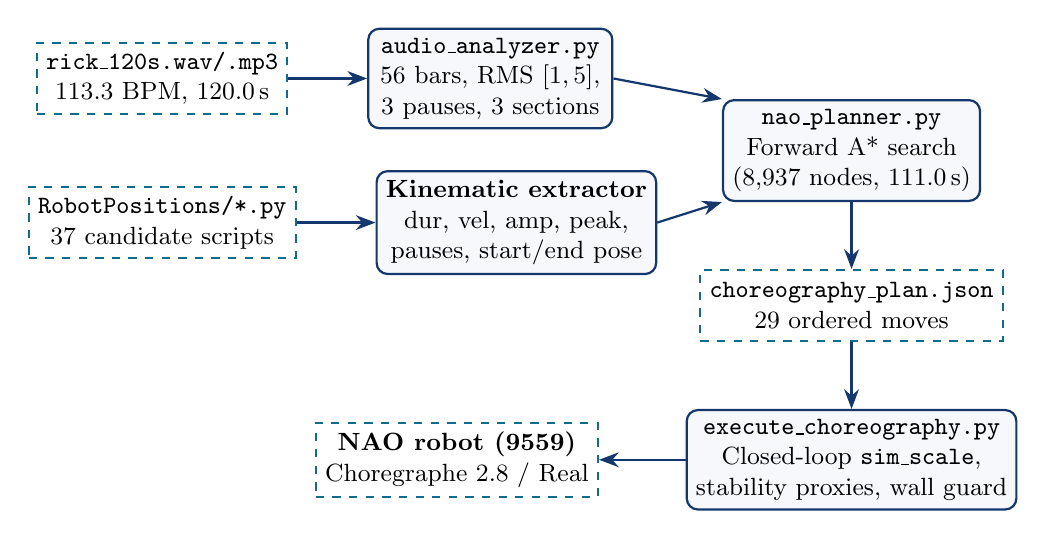
\begin{tikzpicture}[
    node distance=0.85cm and 0.9cm,
    box/.style={rectangle, rounded corners=4pt, draw=navy, fill=lightgraybg, thick, minimum width=3.1cm, minimum height=1.05cm, align=center, font=\small},
    io/.style={rectangle, draw=tealblue, fill=white, dashed, thick, minimum width=2.8cm, minimum height=0.9cm, align=center, font=\small},
    arr/.style={-{Stealth[length=2.5mm]}, thick, navy}
  ]
    \node[io] (audio) {\code{rick\_120s.wav/.mp3}\\113.3 BPM, 120.0\,s};
    \node[io, below=0.9cm of audio] (moves) {\code{RobotPositions/*.py}\\37 candidate scripts};

    \node[box, right=1.0cm of audio] (analyzer) {\textbf{\code{audio\_analyzer.py}}\\56 bars, RMS $[1,5]$,\\3 pauses, 3 sections};
    \node[box, right=1.0cm of moves] (kin) {\textbf{Kinematic extractor}\\dur, vel, amp, peak,\\pauses, start/end pose};

    \node[box, right=1.1cm of $(analyzer.east)!0.5!(kin.east)$] (astar) {\textbf{\code{nao\_planner.py}}\\Forward A* search\\(8,937 nodes, 111.0\,s)};
    \node[io, below=0.85cm of astar] (plan) {\code{choreography\_plan.json}\\29 ordered moves};
    \node[box, below=0.85cm of plan] (exec) {\textbf{\code{execute\_choreography.py}}\\Closed-loop \code{sim\_scale},\\stability proxies, wall guard};
    \node[io, left=1.1cm of exec] (nao) {\textbf{NAO robot (9559)}\\Choregraphe 2.8 / Real};

    \draw[arr] (audio) -- (analyzer);
    \draw[arr] (moves) -- (kin);
    \draw[arr] (analyzer.east) -- (astar.north west);
    \draw[arr] (kin.east) -- (astar.south west);
    \draw[arr] (astar) -- (plan);
    \draw[arr] (plan) -- (exec);
    \draw[arr] (exec) -- (nao);
  \end{tikzpicture}
  \caption{Data flow from audio and move scripts through A* planning to NAO execution.}
  \label{fig:arch}
\end{figure}

\subsection{Audio analysis (\texorpdfstring{\code{audio\_analyzer.py}}{audio\_analyzer.py})}

A dance looks natural when fast moves happen during loud choruses and calmer moves happen during intros or breaks. \code{audio\_analyzer.py} measures this directly from \code{rick\_120s.wav} (120.0\,s, 16-bit PCM WAV) without external audio libraries.

At 113.3\,BPM, one beat lasts $b = 60 / 113.3 \approx 0.52957\,\text{s}$, and a standard 4-beat musical bar lasts $4b = 2.11827\,\text{s}$. Starting from the first downbeat at $\phi = 0.21\,\text{s}$, \code{get\_bar\_features()} splits the song into 56 bars and reads the loudness (RMS amplitude $\text{RMS}_k$) of each beat $k \in \{0,1,2,3\}$. Each bar $j$ gets a normalized energy score $E_j$ from 1.0 (quietest) to 5.0 (loudest):
\[
  \overline{\text{RMS}}_j = \frac{1}{4}\sum_{k=0}^{3}\text{RMS}_k, \qquad
  E_j = 1.0 + 4.0 \cdot \frac{\overline{\text{RMS}}_j - \min_i \overline{\text{RMS}}_i}{\max\big(1.0,\; \max_i \overline{\text{RMS}}_i - \min_i \overline{\text{RMS}}_i\big)}.
\]

Some bars have a sharp drop in volume on one beat, such as a drum break. If any beat falls below 78\% of its bar average ($\min_k \text{RMS}_k < 0.78 \cdot \overline{\text{RMS}}_j$), that bar gets \code{has\_pause = True}. Across \code{rick\_120s.wav}, this flags 3 bars: bar 0 at $t = 0.21\,\text{s}$, bar 13 at $t = 27.75\,\text{s}$, and bar 55 at $t = 116.71\,\text{s}$.

Next, the analyzer groups every 4 consecutive bars (a musical phrase) into sections by average loudness. A phrase joins an existing section $s$ with average energy $c_s$ if $|\bar{e}_{\text{phrase}} - c_s| \le 0.65$; otherwise it starts a new section. On \code{rick\_120s.wav}, this separates the song into 3 sections:
\begin{itemize}[leftmargin=1.5em]
  \item Section 0 (verse and bridge): 24 bars with mean energy $2.94$ (range $2.26$ to $3.64$).
  \item Section 1 (chorus): 24 bars with mean energy $4.56$ (range $4.12$ to $5.00$).
  \item Section 2 (outro fade): 8 bars with mean energy $1.74$ (range $1.00$ to $2.29$).
\end{itemize}
If no WAV file exists, \code{nao\_planner.py} calls \code{get\_energy\_profile()}, which reads MP3 frame payloads in pure Python (\code{\_parse\_mp3\_pure}) or uses a 5-stage fallback curve over 24 slices. When \code{numpy} and \code{scipy.signal} are present, \code{detect\_tempo\_and\_beats()} can also estimate BPM from WAV files in $[80, 160]\,\text{BPM}$.

\subsection{Kinematic feature extraction (\texorpdfstring{\code{nao\_planner.py}}{nao\_planner.py})}

Rather than guessing a score for every dance script by hand, \code{build\_move\_library()} reads the 37 configured move files in \code{RobotPositions/} (1 initial, 1 goal, 6 mandatory, and 29 intermediate moves) and measures how each move actually behaves.

\code{\_parse\_trajectories()} supports three script formats: Choregraphe \code{names.append}/\allowbreak\code{times.append}/\allowbreak\code{keys.append} calls, top-level \code{names}/\allowbreak\code{times}/\allowbreak\code{keys} lists, and procedural \code{t\_grid}/\code{keys} definitions evaluated in a safe local scope (\code{DEG}, \code{list}, \code{round}, \code{range}). Twelve scripts do not use static keyframe tables because they call blocking functions like \code{angleInterpolation()}, \code{setAngles()}, or \code{goToPosture()} directly (the 10 course/official scripts with \code{peak\_vel = 0} and the 2 walks). For those, \code{extract\_move\_features()} reads blocking call timers or uses \code{fallback\_dur} and default speed/amplitude values.

For every parsed script with joint angles $\{(t_{j,i}, k_{j,i})\}$, the extractor measures duration $d$, each joint's total sweep $\text{amp}_j$, its average speed $\text{vel}_j$, and the fastest single jump $\text{peak\_vel}$:
\begin{align*}
  d &= \operatorname{round}\!\left(\max_{j,i} t_{j,i} + \mathbb{I}[\text{\code{goToPosture} in src}],\; 2\right), \\
  \text{amp}_j &= \max_i k_{j,i} - \min_i k_{j,i}, \qquad
  \text{vel}_j = \frac{\sum_{i>0}|k_{j,i}-k_{j,i-1}|}{\max(t_{j,\text{end}}-t_{j,0}, 0.1)}, \\
  \text{peak\_vel} &= \max_{j, i>0} \frac{|k_{j,i}-k_{j,i-1}|}{\max(t_{j,i}-t_{j,i-1}, 0.04)}.
\end{align*}
When the robot waves its arms, its 10 leg joints barely move. Averaging across all joints would make an energetic arm dance look slow, so we average only the upper 50\% most active joints to get \code{raw\_vel} and \code{raw\_amp}. Those numbers are scaled against the 90th percentile across all 37 moves into \code{energy} $\in [1.4, 5.0]$ and \code{expressiveness} $\in [1.5, 5.0]$.

The extractor also records whether legs move (\code{leg\_active}), whether the move holds a pose (\code{has\_pause}, true when all joints change by less than $0.05\,\text{rad}$ over any segment $\Delta t \ge 0.40\,\text{s}$), and each script's first and last joint angles (\code{start\_pose}, \code{end\_pose}). Notice that \code{\_STRIPPED\_LEG\_FILES} lists \code{"finger\_snap.py"} and \code{"DanceMove.py"}; neither script is in the 37-move \code{INTERMEDIATE\_SPECS} pool, so that set sits there as a guard if those files are re-enabled later. To avoid jerky transitions, \code{\_pose\_gap(u, v)} measures how far shared joints $J_u \cap J_v$ have to jump between the end of move $u$ and the start of move $v$:
\[
  \text{\_pose\_gap}(u, v) = \frac{1}{|J_u \cap J_v|} \sum_{j \in J_u \cap J_v} |\text{end\_pose}_u(j) - \text{start\_pose}_v(j)| \quad (\text{default } 0.25\text{ if unparsed}).
\]

\subsection{Forward state-space A* planner (\texorpdfstring{\code{ChoreographyPlanner}}{ChoreographyPlanner})}

\subsubsection{State space and deduplication}
Think of each search node as a snapshot of the choreography at a given moment. The planner stores that snapshot as a 9-tuple:
\[
  s = \big(t,\; \text{mand\_mask},\; \text{pos},\; x,\; y,\; \text{off\_cnt},\; \text{visited\_stage},\; \text{used},\; \text{hist}\big).
\]
In plain terms, the fields track: elapsed time $t$; which of the 6 mandatory moves are done (\code{mand\_mask} packs 6 yes/no checkboxes into an integer from $0$ to $63$); current body posture \code{pos} (\code{Standing}, \code{Sitting}, or \code{Crouch}); current stage grid square $(x,y) \in \{-1,0,1\}^2$; how many distinct official moves ran (\code{off\_cnt}); whether the robot has left center $(0,0)$ yet (\code{visited\_stage}); which intermediate files ran (\code{used}); and the full move list (\code{hist}).

Exploring every tiny timing difference would blow up memory. Within a 120,000-node expansion cap, the planner groups time into 2-second buckets and keeps only the lowest-cost ($f = g + h$) state per bucket:
\[
  \text{key}(s) = \big(\text{mand\_mask},\; \text{pos},\; x,\; y,\; \min(\text{off\_cnt},5),\; \text{visited\_stage},\; \text{last\_mand},\; \operatorname{round}(t / 2.0)\big).
\]

\subsubsection{Goal test and constraints}
Starting from \code{14-StandInit.py} at $t=0.5\,\text{s}$, $\text{pos}=\text{Standing}$, and $(x,y)=(0,0)$, a state is a valid goal when all 6 mandatory moves are done ($\text{mand\_mask}=63$), the robot is standing at center $(0,0)$ after visiting another cell, at least 5 official moves ran, and elapsed time sits between $109.0\,\text{s}$ and $115.0 - d_{\text{crouch}}$:
\begin{align*}
  \text{mand\_mask} = 63 \;\wedge\; \text{pos} = \text{Standing} \;\wedge\; (x, y) = (0, 0) \\
  \wedge\; \text{visited\_stage} \;\wedge\; \text{off\_cnt} \ge 5 \;\wedge\; 109.0 \le t \le 115.0 - d_{\text{crouch}}.
\end{align*}
Once that holds, \code{6-Crouch.py} ($d_{\text{crouch}}=1.8\,\text{s}$) is added at the end. Six rules block illegal moves during expansion:
\begin{enumerate}[leftmargin=1.5em]
  \item Every move must match the current posture (\code{pre == pos}).
  \item Mandatory moves cannot run consecutively while \code{Standing} (\code{last\_mand} guard), forcing dance moves between standing milestones while allowing the floor chain \code{16-Sit} $\to$ \code{17-SitRelax} $\to$ \code{11-Stand}.
  \item \code{16-Sit.py} requires stage center $(0,0)$, and \code{11-Stand.py} cannot run before \code{17-SitRelax.py}.
  \item No move can repeat immediately back to back, and two leg-static standing intermediate moves cannot run in a row. Repetition caps allow at most 3 plays for bar-locked ($\text{beat\_err} < 0.08\,\text{s}$) leg-active moves $\le 4.3\,\text{s}$, 2 plays for other leg-active moves $\le 6.0\,\text{s}$, and 1 play for walks, moves $>6.0\,\text{s}$, or leg-static moves.
  \item Coordinates must stay inside $|x| \le 1$, $|y| \le 1$. Once $t \ge 101.0\,\text{s}$ (\code{max\_duration - 14.0}), any move with $|x'| > |x|$ or $|y'| > |y|$ is rejected.
  \item Any expansion where $t' + d_{\text{rem\_mand}} + d_{\text{crouch}} > 115.0\,\text{s}$ is pruned.
\end{enumerate}

\subsubsection{Cost function, heuristic, and admissibility}
A* searches for the path with the lowest total cost. If good moves had negative costs, the planner would stuff extra filler moves into the routine just to push the total down. Instead, we turn every reward into a positive "regret" penalty, scaled by move length $d_m / 4.24$ and floored at $0.3$:
\begin{align*}
  \text{cost}_{\text{mand}}(m, t) &= \max\!\left(0.3,\; \Big(2.5 + 3.0\,|E_m - E_{\text{target}}(t)|\Big)\frac{d_m}{4.24}\right), \\
  \text{cost}_{\text{inter}}(m, t) &= \max\!\Big(0.3,\; \big(12.0 - \text{expr}_m - \text{body}_m - \text{pause}_m - \text{off}_m - \text{repeat}_m \\
  &\qquad\qquad\qquad {} + 2.0\,e_{\text{err}} + 4.5\,\text{beat\_err} + \text{jerk}_m + 2.5\,\text{pose\_gap}\big)\frac{d_m}{4.24}\Big).
\end{align*}
Good qualities lower the penalty inside the parentheses: wide expression ($\text{expr}_m$), leg movement ($\text{body}_m = 2.0$), matching a musical pause ($\text{pause}_m = 2.0$), unlocking a needed official move ($\text{off}_m = 2.5$), or repeating a non-walk hook inside the same song section ($\text{repeat}_m = 2.6$). Bad qualities raise the penalty: energy mismatch $e_{\text{err}}$, off-bar duration $\text{beat\_err} = \min(d_m \bmod \text{bar},\; \text{bar} - (d_m \bmod \text{bar}))$, velocity spikes $\text{jerk}_m = 0.8 \cdot \max(0, \text{peak\_vel}_m - 4.5)$, and joint jumps $\text{pose\_gap}$.

The heuristic $h(s)$ estimates the remaining penalty for unfinished mandatory moves ($\text{rem}_m$), missing official moves ($\text{rem}_o$), walking back to $(0,0)$, standing up from sitting, and filling time up to $109.0\,\text{s}$:
\begin{align*}
  h(s) &= 4.0\,\text{rem}_m + 3.5\,\text{rem}_o + 2.5(|x| + |y|) \\
       &\quad {} + 2.5\,\mathbb{I}[\neg\text{visited\_stage}] + 2.0\,\mathbb{I}[\text{pos} = \text{Sitting}] + 1.55\,\max(0,\; 109.0 - t).
\end{align*}

\paragraph{Admissibility and optimality.}
Our heuristic $h(s)$ is weighted and not admissible. Each remaining second until $109.0\,\text{s}$ adds $1.55$ to $h(s)$, while a cheap step can cost as little as $0.3$ over $4.24\,\text{s}$ ($0.071/\text{s}$). Combined with $2.0\,\text{s}$ time buckets, A* trades a strict guarantee of the single lowest global cost for speed: \code{solve()} finishes in 8,937 nodes ($0.077\,\text{s}$) while checking every hard rule on every step.

\subsection{Execution engine and simulator stabilization (\texorpdfstring{\code{execute\_choreography.py}}{execute\_choreography.py})}

Rather than editing 37 official and course scripts, \code{execute\_choreography.py} swaps \code{naoqi.ALProxy} at runtime. Every script reuses one connection per NAOqi service without changing the original files.

\paragraph{Closed-loop beat sync.}
Choregraphe often runs slower than real time on a laptop ($0.63\times$ to $0.77\times$ speed during our live test). If we played timestamps blindly, the robot would fall behind the music. \code{\_SyncedMotionProxy} acts like a feedback loop: for blocking keyframe moves lasting at least $1.5\,\text{s}$ (\code{is\_beat\_move}), it pulls the expected end time within $\pm 1$ beat of \code{target\_end}, snaps the end to the nearest beat ($\phi + k\cdot b$), and scales timestamps by \code{sim\_scale}. \code{\_scale\_times()} keeps at least $0.16\,\text{s}$ between consecutive timestamps per joint (and $0.18\,\text{s}$ minimum first keyframe) so motors do not trigger velocity errors. Scalar-time calls scale by \code{sim\_scale} without beat snapping. Whenever wall time and sent time exceed $0.5\,\text{s}$, an exponential moving average ($\alpha = 0.45$, clamped to $[0.62, 1.05]$) updates \code{sim\_scale}. Before intermediate moves, a short wait ($0.02 < \text{wait} \le 0.28\,\text{s}$) starts the step on the beat, and module-level keyframe files shift their first keyframe to at least $0.45\,\text{s}$.

\paragraph{Floor and sitting stabilization.}
As noted in \code{execute\_choreography.py}, stock \code{ALRobotPosture.goToPosture} calls for \code{Sit} and \code{SitRelax} can hit the virtual floor or tip the robot backward inside Choregraphe, stalling for up to 30\,s in fall recovery. \code{\_FastPostureProxy} replaces \code{Sit} with verified joint arrays (\code{\_CROUCH\_ANGLES} for 1.2\,s, then \code{\_SIT\_ANGLES} for 2.2\,s) and replaces \code{SitRelax} with \code{\_SITRELAX\_ANGLES} (2.5\,s). When standing up via \code{11-Stand.py}, it first tucks into \code{\_CROUCH\_ANGLES} over 1.6\,s so the center of mass sits over the feet, then calls \code{self.\_real.goToPosture(postureName, 0.9)}. An isolated test on port 9559 confirmed that \code{SitRelax} $\to$ \code{Crouch} $\to$ \code{Stand} lands upright in \code{Posture = Stand} at \code{HeadZ = 0.458\,m}. For standing moves in \code{["finger\_snap", "DanceMove"]} or floor scripts with \code{"sitting"} in the filename, the executor also strips \code{Hip}, \code{Knee}, and \code{Ankle} tracks.

\paragraph{Targeted sleep patch, wall guard, and CLI.}
Course files call \code{ttsProxy.say(...)} followed by \code{time.sleep(1)}. \code{\_DummyTTS.say()} sets \code{\_SYNC\_STATE["skip\_next\_sleep"] = True} (reset before each move) so \code{\_fluid\_sleep} skips only that 1\,s speech pause. Real motion waits ($\ge 0.1\,\text{s}$) inside \code{setAngles()} scripts like \code{3-Double\_movement.py} and \code{4-Arms\_opening.py} still run, scaled by $0.5$ and capped at $1.0\,\text{s}$. During the loop, \code{MAX\_WALL\_TIME = 115.5\,s} skips late non-official, non-displacement moves if \code{elapsed\_now + est\_dur > 115.5\,s}, leaving mandatory and official steps intact. Audio plays via Windows \code{winmm} MCI (with PowerShell fallback), macOS \code{afplay}, or Linux \code{mpg123}, and the CLI accepts \code{[port]}, \code{[ip]}, \code{[ip] [port]}, \code{dry\_run}, \code{--ip}, \code{--port}/\code{-p}, and \code{--music}/\code{-m}.

\clearpage

% ----------------------------------------------------------------------
% SECTION 4: GENERATED CHOREOGRAPHY AND VERIFICATION
% ----------------------------------------------------------------------
\section{Generated choreography and experimental verification}

\subsection{Planned 29-step sequence and live Choregraphe trace}

Table~\ref{tab:plan} shows all 29 steps in \code{choreography\_plan.json} next to the wall-clock timestamps recorded during our live run on Choregraphe Suite 2.8 (\code{127.0.0.1 9559 --music \_\_none\_\_}).

{\footnotesize
\setlength{\tabcolsep}{4pt}
\begin{longtable}{r c l l c r r l}
  \caption{Planned 29-step choreography (111.0\,s) vs.\ live Choregraphe 2.8 run (115.4\,s).} \label{tab:plan} \\
  \toprule
  \textbf{\#} & \textbf{Sec} & \textbf{Type} & \textbf{Move script} & \textbf{Off.} & \textbf{Plan (s)} & \textbf{Cum (s)} & \textbf{Live $t$ (s)} \\
  \midrule
  \endfirsthead
  \toprule
  \textbf{\#} & \textbf{Sec} & \textbf{Type} & \textbf{Move script} & \textbf{Off.} & \textbf{Plan (s)} & \textbf{Cum (s)} & \textbf{Live $t$ (s)} \\
  \midrule
  \endhead
  \bottomrule
  \endfoot
  1  & 0 & INITIAL      & \code{14-StandInit.py}        & No  & 0.50  & 0.5   & 0.3 \\
  2  & 0 & MANDATORY    & \code{WipeForehead.py}        & Yes & 6.00  & 6.5   & 7.7 \\
  3  & 0 & INTERMEDIATE & \code{3-Double\_movement.py}  & Yes & 4.40  & 10.9  & 14.7 \\
  4  & 1 & MANDATORY    & \code{Hello.py}               & Yes & 5.60  & 16.5  & 20.3 \\
  5  & 1 & INTERMEDIATE & \code{sprinkler.py}           & Yes & 10.40 & 26.9  & 30.3 \\
  6  & 0 & MANDATORY    & \code{15-StandZero.py}        & Yes & 1.40  & 28.3  & 31.8 \\
  7  & 0 & INTERMEDIATE & \code{motif\_disco\_point.py} & No  & 4.24  & 32.5  & 36.1 \\
  8  & 0 & MANDATORY    & \code{16-Sit.py}              & Yes & 3.50  & 36.0  & 39.5 \\
  9  & 0 & MANDATORY    & \code{17-SitRelax.py}         & Yes & 2.50  & 38.5  & 42.0 \\
  10 & 0 & MANDATORY    & \code{11-Stand.py}            & Yes & 3.30  & 41.8  & 46.2 \\
  11 & 0 & INTERMEDIATE & \code{motif\_disco\_point.py} & No  & 4.24  & 46.1  & 50.2 \\
  12 & 0 & INTERMEDIATE & \code{motif\_beat\_drop.py}   & No  & 2.12  & 48.2  & 52.3 \\
  13 & 0 & INTERMEDIATE & \code{motif\_disco\_point.py} & No  & 4.24  & 52.4  & 56.4 \\
  14 & 1 & INTERMEDIATE & \code{dab.py}                 & No  & 4.64  & 57.1  & 61.0 \\
  15 & 1 & INTERMEDIATE & \code{4-Arms\_opening.py}     & Yes & 5.00  & 62.1  & 69.4 \\
  16 & 1 & INTERMEDIATE & \code{dab.py}                 & No  & 4.64  & 66.7  & 74.0 \\
  17 & 1 & INTERMEDIATE & \code{8-Move\_backward.py}    & Yes & 3.50  & 70.2  & 78.6 \\
  18 & 1 & INTERMEDIATE & \code{ThrillerClap.py}        & No  & 5.00  & 75.2  & 83.4 \\
  19 & 1 & INTERMEDIATE & \code{motif\_pop\_clap.py}    & No  & 2.12  & 77.3  & 85.5 \\
  20 & 1 & INTERMEDIATE & \code{ThrillerClap.py}        & No  & 5.00  & 82.3  & 90.1 \\
  21 & 1 & INTERMEDIATE & \code{motif\_finger\_snap.py} & No  & 4.24  & 86.6  & 94.3 \\
  22 & 0 & INTERMEDIATE & \code{7-Move\_forward.py}     & Yes & 3.50  & 90.1  & 100.6 \\
  23 & 0 & INTERMEDIATE & \code{motif\_astley\_groove.py}& No & 4.24  & 94.3  & 104.8 \\
  24 & 0 & INTERMEDIATE & \code{motif\_beat\_drop.py}   & No  & 2.12  & 96.4  & 107.2 \\
  25 & 0 & INTERMEDIATE & \code{motif\_astley\_groove.py}& No & 4.24  & 100.7 & 111.3 \\
  26 & 0 & INTERMEDIATE & \code{motif\_beat\_drop.py}   & No  & 2.12  & 102.8 & 113.4 \\
  27 & 2 & INTERMEDIATE & \code{motif\_astley\_groove.py}& No & 4.24  & 107.0 & Skipped (wall guard) \\
  28 & 2 & INTERMEDIATE & \code{motif\_groove\_pause.py}& No  & 2.12  & 109.2 & Skipped (wall guard) \\
  29 & 2 & GOAL         & \code{6-Crouch.py}            & Yes & 1.80  & 111.0 & 115.4 \\
\end{longtable}
}

\clearpage
\subsection{Kinematic profile of selected moves}

Table~\ref{tab:kin} gives the measured kinematic values for the 21 distinct moves in \code{choreography\_plan.json}. Scripts without explicit trajectory arrays show \code{Peak vel = 0.00} and use blocking call parsing or \code{fallback\_dur}.

\begin{table}[H]
  \centering
  \scriptsize
  \setlength{\tabcolsep}{4.2pt}
  \caption{Extracted kinematic values for the 21 distinct moves in \code{choreography\_plan.json}.}
  \label{tab:kin}
  \begin{tabular}{l r r r r r r c c l}
    \toprule
    \textbf{Move file} & \textbf{Dur (s)} & \textbf{Raw vel} & \textbf{Raw amp} & \textbf{Peak vel} & \textbf{Energy} & \textbf{Expr.} & \textbf{Leg} & \textbf{Pause} & \textbf{Role} \\
    \midrule
    \code{14-StandInit.py}         &  0.50 & 0.25 & 0.60 & 0.00 & 1.8 & 2.8 & No  & No  & Initial \\
    \code{WipeForehead.py}         &  6.00 & 0.36 & 0.89 & 2.14 & 2.6 & 3.9 & No  & Yes & Mandatory \\
    \code{3-Double\_movement.py}   &  4.40 & 0.45 & 0.70 & 0.00 & 3.2 & 3.2 & No  & No  & Official int. \\
    \code{Hello.py}                &  5.60 & 0.54 & 1.01 & 2.04 & 3.8 & 4.3 & No  & Yes & Mandatory \\
    \code{sprinkler.py}            & 10.40 & 0.74 & 1.31 & 3.00 & 5.0 & 5.0 & Yes & Yes & Official int. \\
    \code{15-StandZero.py}         &  1.40 & 0.25 & 0.60 & 0.00 & 1.8 & 2.8 & No  & No  & Mandatory \\
    \code{motif\_disco\_point.py}  &  4.24 & 0.42 & 1.00 & 3.93 & 3.0 & 4.3 & Yes & Yes & Extra int. \\
    \code{16-Sit.py}               &  3.50 & 0.25 & 0.60 & 0.00 & 1.8 & 2.8 & No  & No  & Mandatory \\
    \code{17-SitRelax.py}          &  2.50 & 0.25 & 0.60 & 0.00 & 1.8 & 2.8 & No  & No  & Mandatory \\
    \code{11-Stand.py}             &  3.30 & 0.25 & 0.60 & 0.00 & 1.8 & 2.8 & No  & No  & Mandatory \\
    \code{motif\_beat\_drop.py}    &  2.12 & 0.41 & 0.60 & 2.73 & 2.9 & 2.8 & Yes & Yes & Extra int. \\
    \code{dab.py}                  &  4.64 & 0.69 & 1.43 & 2.56 & 4.9 & 5.0 & Yes & No  & Extra int. \\
    \code{4-Arms\_opening.py}      &  5.00 & 0.45 & 0.70 & 0.00 & 3.2 & 3.2 & No  & No  & Official int. \\
    \code{8-Move\_backward.py}     &  3.50 & 0.28 & 0.45 & 0.00 & 2.0 & 2.2 & Yes & No  & Official int. \\
    \code{ThrillerClap.py}         &  5.00 & 0.66 & 1.18 & 1.98 & 4.6 & 5.0 & Yes & Yes & Extra int. \\
    \code{motif\_pop\_clap.py}     &  2.12 & 1.38 & 0.72 & 3.31 & 5.0 & 3.2 & No  & No  & Extra int. \\
    \code{motif\_finger\_snap.py}  &  4.24 & 0.70 & 0.83 & 4.21 & 4.9 & 3.7 & No  & No  & Extra int. \\
    \code{7-Move\_forward.py}      &  3.50 & 0.28 & 0.45 & 0.00 & 2.0 & 2.2 & Yes & No  & Official int. \\
    \code{motif\_astley\_groove.py}&  4.24 & 0.32 & 0.61 & 1.15 & 2.3 & 2.9 & Yes & Yes & Extra int. \\
    \code{motif\_groove\_pause.py} &  2.12 & 0.21 & 0.26 & 1.56 & 1.5 & 1.5 & Yes & Yes & Extra int. \\
    \code{6-Crouch.py}             &  1.80 & 0.25 & 0.60 & 0.00 & 1.8 & 2.8 & No  & No  & Goal \\
    \bottomrule
  \end{tabular}
\end{table}

The kinematic measurements show clear separation across the move catalog. Expressive moves like \code{sprinkler.py} and \code{dab.py} reach the maximum score of 5.0 in energy and expressiveness, with leg movements and wide joint sweeps (raw amplitude $> 1.30\,\text{rad}$). Static milestone poses such as \code{15-StandZero.py} and floor transitions show baseline scores ($1.8$ energy, $2.8$ expressiveness). By combining these values with musical section loudness, the A* planner places high-energy moves in the chorus and keeps calmer transitions in quieter verses.

\clearpage

% ----------------------------------------------------------------------
% SECTION 5: DESIGN DECISIONS AND TRADE-OFFS
% ----------------------------------------------------------------------
\section{Design decisions and trade-offs}

Designing an autonomous choreography planner for a humanoid robot requires balancing multiple competing constraints: temporal precision, kinematic smoothness, search efficiency, and simulator stability. Table~\ref{tab:decisions} summarizes our key architectural choices, the alternatives we evaluated, and the rationale behind each trade-off.

\begin{table}[H]
  \centering
  \scriptsize
  \caption{Summary of architectural choices, alternatives, and trade-offs.}
  \label{tab:decisions}
  \begin{tabularx}{\textwidth}{>{\raggedright\arraybackslash}p{2.5cm} >{\raggedright\arraybackslash}p{2.8cm} >{\raggedright\arraybackslash}p{2.8cm} X}
    \toprule
    \textbf{Decision} & \textbf{Chosen design} & \textbf{Alternative} & \textbf{Rationale and trade-off} \\
    \midrule
    Search algorithm & Custom Python forward A* & External PDDL planner or Simulated Annealing & PDDL does not handle continuous time, audio bar lookup, and pose gaps natively; Simulated Annealing varies across runs. Python A* solves deterministically in 8,937 nodes. \\
    Mandatory ordering & Dynamic 6-bit mask & Fixed $P_1 \to \dots \to P_6$ sequence & Lets A* put \code{WipeForehead} in the intro, \code{Hello} in Section 1, and \code{16-Sit} $\to$ \code{17-SitRelax} $\to$ \code{11-Stand} in order while keeping all 6 required. \\
    Move scoring & Auto-extracted joint kinematics & Hand-authored score table & Ties scores to actual joint speed, amplitude, and end/start angles with no manual tuning table. \\
    Heuristic tightness & Weighted $h(s)$ with 2\,s buckets & Strictly admissible $h(s)$ & Solves in 0.077\,s inside the 120,000-node cap; gives up strict global cost optimality. \\
    Reward formulation & Positive regret floored at 0.3 & Raw negative rewards & Prevents min-heap loops and stops the planner from stretching cheap moves just to fill time. \\
    Script adaptation & Runtime \code{ALProxy} wrapping & Editing \code{RobotPositions/}\allowbreak\code{*.py} & Leaves course and official files untouched so they still run standalone, at the cost of proxy indirection. \\
    Floor transitions & Direct joint arrays plus \code{Crouch} tuck & Stock \code{ALRobotPosture} IK & Avoids virtual floor collisions and backward tipping seen in Choregraphe; hardcodes NAO H25 angles in \code{execute\_choreography.py}. \\
    Timing model & Closed-loop \code{sim\_scale} plus wall guard & Static open-loop timing & Absorbs simulator slowdown ($0.63\times$ to $0.77\times$); skips Steps 27 and 28 at 113.4\,s to keep total run under 120\,s. \\
    Audio stack & Stdlib WAV/MP3 parser & \code{librosa}, \code{pydub}, or \code{ffmpeg} & Zero third-party dependencies for graders; defaults WAV bar detection to 113.3\,BPM unless \code{numpy} is wired in. \\
    \bottomrule
  \end{tabularx}
\end{table}

\clearpage

% ----------------------------------------------------------------------
% SECTION 6: PRESENTATION AND ORAL DEFENSE Q&A
% ----------------------------------------------------------------------
\section{Presentation and oral-defense Q\&A}

\subsection*{A. AI planning and search theory}

\begin{qa}{Q1. Why write forward A* in Python instead of using a PDDL planner or Simulated Annealing?}
PDDL handles boolean preconditions well, but it cannot evaluate continuous time ($109.0 \le t \le 115.0\,\text{s}$), sliding bar-by-bar loudness lookup, bar modulo beat error, or shared-joint pose gaps out of the box. Simulated Annealing gives different plans on different runs unless seeded. Forward A* in Python handles temporal and audio costs directly, checks every rule at every step, and solves the 37-move pool deterministically in 8,937 nodes (0.077\,s).
\end{qa}

\begin{qa}{Q2. Is your heuristic $h(s)$ admissible or consistent?}
No. It is a weighted, non-admissible heuristic. Each missing second before $109.0\,\text{s}$ adds $1.55$ to $h(s)$, while a cheap step can cost as little as $0.3$ over $4.24\,\text{s}$ ($0.071/\text{s}$). Overestimating remaining cost turns the search into weighted A*, pushing expansions toward the $109.0\,\text{s}$ minimum duration quickly instead of hitting the 120,000-node cap. Every hard rule (mandatory mask $=63$, $\ge 5$ official moves, posture legality, center return, $T \le 115\,\text{s}$) is checked in the goal test, so the output plan is always valid.
\end{qa}

\begin{qa}{Q3. Why use positive regret instead of maximizing positive reward directly?}
A* uses a min-heap ordered by $f = g + h$ and expects non-negative step costs. Subtracting rewards directly creates negative edges, which makes longer paths look cheaper and encourages filler loops. Flooring every step cost at $0.3$ and scaling by $d_m / 4.24$ ensures $g$ rises as time passes.
\end{qa}

\begin{qa}{Q4. Why quantize time as \code{round(t / 2.0)} in the visited dictionary?}
Move durations differ slightly ($2.12\,\text{s}$, $3.50\,\text{s}$, $4.24\,\text{s}$, $4.64\,\text{s}$, $5.00\,\text{s}$). Keeping exact floating-point timestamps would treat schedules differing by $0.05\,\text{s}$ as separate states and explode the search tree. Grouping states into 2-second buckets (about one bar) keeps only the cheapest representative per bucket.
\end{qa}

\begin{qa}{Q5. How do you model consecutive move incompatibilities (Slide 14)?}
Incompatibilities are blocked at three levels. Posture rules (\code{Standing}, \code{Sitting}, \code{Crouch}) stop standing scripts from running during seated phases. Floor rules force \code{16-Sit} at $(0,0)$ and require \code{11-Stand} after \code{17-SitRelax}. Search guards also block consecutive identical moves, consecutive leg-static standing moves, and sharp joint jumps via \code{\_pose\_gap} and \code{peak\_vel} penalties.
\end{qa}

\begin{qa}{Q6. Why schedule the 6 mandatory positions with a bitmask instead of fixing the order $P_1$ through $P_6$?}
Slide 13 lists the 6 required milestones (\code{Sit}, \code{SitRelax}, \code{WipeForehead}, \code{Stand}, \code{Hello}, \code{StandZero}) without prescribing one permutation. Using a 6-bit mask lets the planner place \code{WipeForehead} in the quieter intro (Section 0), put \code{Hello} at the louder chorus entry (Section 1), and run \code{16-Sit} $\to$ \code{17-SitRelax} $\to$ \code{11-Stand} together while finishing all 6 before \code{6-Crouch}.
\end{qa}

\begin{qa}{Q7. How do you stop the 5 official intermediate moves from clumping together (Slide 15)?}
The \code{last\_mand} flag blocks back-to-back standing mandatory moves, forcing dance moves between them. \code{off\_bonus = 2.5} rewards picking each distinct official move until 5 are reached, and energy matching plus \code{\_pose\_gap} spread the 5 chosen official moves across Steps 3, 5, 15, 17, and 22.
\end{qa}

\subsection*{B. Audio analysis and rhythm synchronization}

\begin{qa}{Q8. Does the system work on other songs besides \emph{Never Gonna Give You Up}?}
You can pass any track with \code{--music <file>}. \code{audio\_analyzer.py} reads duration and energy profiles from arbitrary WAV or MP3 files using Python's standard library. One current limitation is that \code{load\_real\_energy\_profile()} calls \code{get\_bar\_features()} without passing an estimated BPM, so WAV files default to $\text{BPM} = 113.3$ and $\phi = 0.21\,\text{s}$. \code{detect\_tempo\_and\_beats()} already has a WAV autocorrelation BPM estimator using \code{numpy} and \code{scipy}, so passing its output into \code{get\_bar\_features()} is the only change needed for other tempos. MP3-only inputs fall back to \code{get\_energy\_profile()}.
\end{qa}

\begin{qa}{Q9. Why keep both \code{rick\_120s.mp3} and \code{rick\_120s.wav}?}
\code{rick\_120s.wav} holds uncompressed 16-bit PCM samples, so \code{audio\_analyzer.py} can compute exact per-beat loudness using Python's built-in \code{wave} module without \code{ffmpeg} or \code{librosa}. \code{rick\_120s.mp3} is much smaller and plays cleanly through Windows MCI, \code{mpg123}, or \code{afplay} during execution.
\end{qa}

\begin{qa}{Q10. Why reward repeating a move inside the same musical section (\code{repeat\_bonus = 2.6})?}
Pop songs repeat musical phrases across verses and choruses, so bringing back a signature move inside the same section makes the dance look structured. In our plan, this repeats \code{motif\_disco\_point} in Section 0 (Steps 7, 11, 13), \code{dab} and \code{ThrillerClap} in Section 1 (Steps 14, 16 and 18, 20), and \code{motif\_astley\_groove} with \code{motif\_beat\_drop} in late Section 0 (Steps 23 to 26). Repetition caps and the back-to-back ban keep it from getting repetitive.
\end{qa}

\begin{qa}{Q11. How do you keep the robot in sync when Choregraphe runs slower than real time?}
In our live run on port 9559, \code{sim\_scale} tracked simulator speed between $0.63$ and $0.77$. At around $0.65\times$ real time, an unscaled $111.0\,\text{s}$ plan would finish well past the $120\,\text{s}$ deadline. \code{\_SyncedMotionProxy} adjusts timing as it goes: it scales timestamps by the online \code{sim\_scale} EMA, snaps \code{is\_beat\_move} endings to the nearest 113.3\,BPM beat with a $\pm 1$-beat drift pull toward \code{target\_end}, and enforces \code{MAX\_WALL\_TIME = 115.5\,s}.
\end{qa}

\subsection*{C. Robotics, kinematics, and simulation stability}

\begin{qa}{Q12. Why did default \code{16-Sit}, \code{17-SitRelax}, and \code{11-Stand} fail in Choregraphe, and how did you fix them?}
As noted in \code{execute\_choreography.py}, stock \code{ALRobotPosture.goToPosture} transitions for \code{Sit} and \code{SitRelax} can hit the virtual floor or tip backward in Choregraphe, stalling for up to 30\,s in recovery, and rising straight from \code{SitRelax} can make the feet slip forward. \code{\_FastPostureProxy} bypasses stock IK on \code{Sit} and \code{SitRelax} with verified joint arrays (\code{\_CROUCH\_ANGLES}, \code{\_SIT\_ANGLES}, \code{\_SITRELAX\_ANGLES}). Before \code{11-Stand} calls \code{goToPosture("Stand", 0.9)}, it tucks into \code{\_CROUCH\_ANGLES} over $1.6\,\text{s}$ to center weight over the feet. A direct test on port 9559 confirmed that \code{SitRelax} $\to$ \code{Crouch} $\to$ \code{Stand} finished upright in \code{Posture = Stand} at \code{HeadZ = 0.458\,m}.
\end{qa}

\begin{qa}{Q13. Why wrap \code{ALProxy} and \code{time.sleep} instead of editing \code{RobotPositions/*.py}?}
Wrapping \code{naoqi.ALProxy} inside \code{execute\_choreography.py} leaves all 37 candidate scripts unchanged so they still run standalone, while letting the executor reuse sockets, mute \code{ALTextToSpeech}, apply beat-sync scaling, and stabilize posture calls in one place. Setting \code{\_SYNC\_STATE["skip\_next\_sleep"] = True} inside \code{\_DummyTTS.say()} skips only the 1\,s pause after speech prompts while keeping scaled motion delays ($\min(0.5 \cdot \text{secs}, 1.0)$) for \code{setAngles()} scripts like \code{3-Double\_movement.py} and \code{4-Arms\_opening.py}.
\end{qa}

\begin{qa}{Q14. Steps 27 and 28 were skipped at 113.4\,s in the live test. Is that a bug?}
No, that is the \code{MAX\_WALL\_TIME = 115.5\,s} guard doing its job. Under Choregraphe load, \code{3-Double\_movement} took $6.98\,\text{s}$ and \code{4-Arms\_opening} took $8.32\,\text{s}$, bringing elapsed wall time to $113.4\,\text{s}$ after Step 26. Because the guard protects mandatory and official moves while skipping late non-official, non-displacement moves, it skipped Steps 27 and 28 (\code{motif\_astley\_groove} and \code{motif\_groove\_pause}) and ran Step 29 (\code{6-Crouch.py}) right away, finishing at 115.4\,s.
\end{qa}

\begin{qa}{Q15. Would the same code run on a real physical NAO robot?}
Yes, using \code{execute\_choreography.py <ROBOT\_IP> 9559}. Because \code{sim\_scale} updates from measured step times and stays within $[0.62, 1.05]$, real-time hardware execution naturally pushes \code{sim\_scale} toward $1.0$. Keyframe sanitization ($\ge 0.16\,\text{s}$ interval between points) already checks joint velocity limits, though sitting and crouch transitions should be tested on a mat before a stage demo.
\end{qa}

\subsection*{D. Artistic criteria, limitations, and extensions}

\begin{qa}{Q16. Why does the final plan only move backward and forward once ($\pm 8\,\text{cm}$)?}
The official walk moves (\code{7-Move\_forward}, \code{8-Move\_backward}) shift $0.08\,\text{m}$ per call, and the goal test only asks for \code{visited\_stage = True} (leaving $(0,0)$ at least once) before returning to center. Walking moves also score lower on \code{expressiveness} ($2.2$) and have durations ($3.5\,\text{s}$) that do not line up with the $2.12\,\text{s}$ bar, so A* visits $(-1,0)$ once via \code{8-Move\_backward} (Step 17) and returns via \code{7-Move\_forward} (Step 22). Giving a bonus for visiting multiple grid squares would produce wider stage movement.
\end{qa}

\begin{qa}{Q17. Do you control NAO's eye, ear, or chest LEDs?}
No. The current code focuses on planning, timing, and physical stability and does not call \code{ALLeds}. Adding \code{ALLeds.post.fadeRGB} calls inside \code{execute\_choreography.py} on move or beat boundaries is a small, optional change if lighting effects are wanted for voting day.
\end{qa}

\begin{qa}{Q18. How does this project connect to Unibo's \emph{Performing Robots} research?}
As described in Slides 9, 11, and 22 of \code{NAOPlanningChallenge2627.pdf}, Unibo's \emph{Performing Robots} project (\code{site.unibo.it/performingrobots/en}) studies automatic generation of robotic dance, using the voting-day survey questions and student choreographies to build a dataset for neural artistic evaluation. Our system maps those seven survey criteria into measurable audio features (bar energy, pauses, sections) and physical joint features (velocity, amplitude, pose continuity, leg movement).
\end{qa}

\begin{qa}{Q19. What keeps the robot from looking stiff between moves?}
Four choices reduce stiffness: the four full-body custom motifs (\code{motif\_astley\_groove}, \code{motif\_disco\_point}, \code{motif\_beat\_drop}, \code{motif\_groove\_pause}) use coordinated knee-bounce, hip-roll, and ankle angles that return to a common neutral stance; \code{\_pose\_gap} penalizes sharp joint jumps between consecutive moves; \code{\_fluid\_sleep} cuts 1\,s post-TTS gaps between scripts; and module-level keyframe files shift their first keyframe to at least $0.45\,\text{s}$ to blend smoothly from the previous pose.
\end{qa}

\end{document}
